\chapter*{Príloha B: Triangulácia a výsledky merania niektorých ďalších plôch}
\label{priloha:prilohaB}
\addcontentsline{toc}{chapter}{Príloha B}


\renewcommand{\arraystretch}{1}
\setlength{\fboxsep}{2mm} % box size
\setlength{\tabcolsep}{-4pt}

V tejto prílohe uvádzame merania kritérii kvality niektorých ďalších konečných plôch, 
aj nekonečných plôch s využitím ohraničujúcej obálky.

\newpage
\section{Konečné plochy}
\begin{enumerate}
\item{
    \textit{Sféra}
    \begin{equation}
    \label{eq:sphere}
    x^2 + y^2 + z^2 - 1 = 0
    \end{equation}

    Na obrázku \ref{obr:sphere} vidíme výslednú trianguláciu sféry danej implicitnou 
    rovnicou \ref{eq:sphere} s piatimi rôznymi dĺžkami strany $a$.
    \begin{enumerate}[a)]
    \item{
        $a=0.900$, $n=64$, $p=34$
    }
    \item{
        $a=0.700$, $n=90$, $p=47$
    }
    \item{
        $a=0.500$, $n=160$, $p=82$
    }
    \item{
        $a=0.300$, $n=408$, $p=206$
    }
    \item{
        $a=0.100$, $n=3246$, $p=1625$
    }
    \end{enumerate}

    \begin{figure}
        \centerline{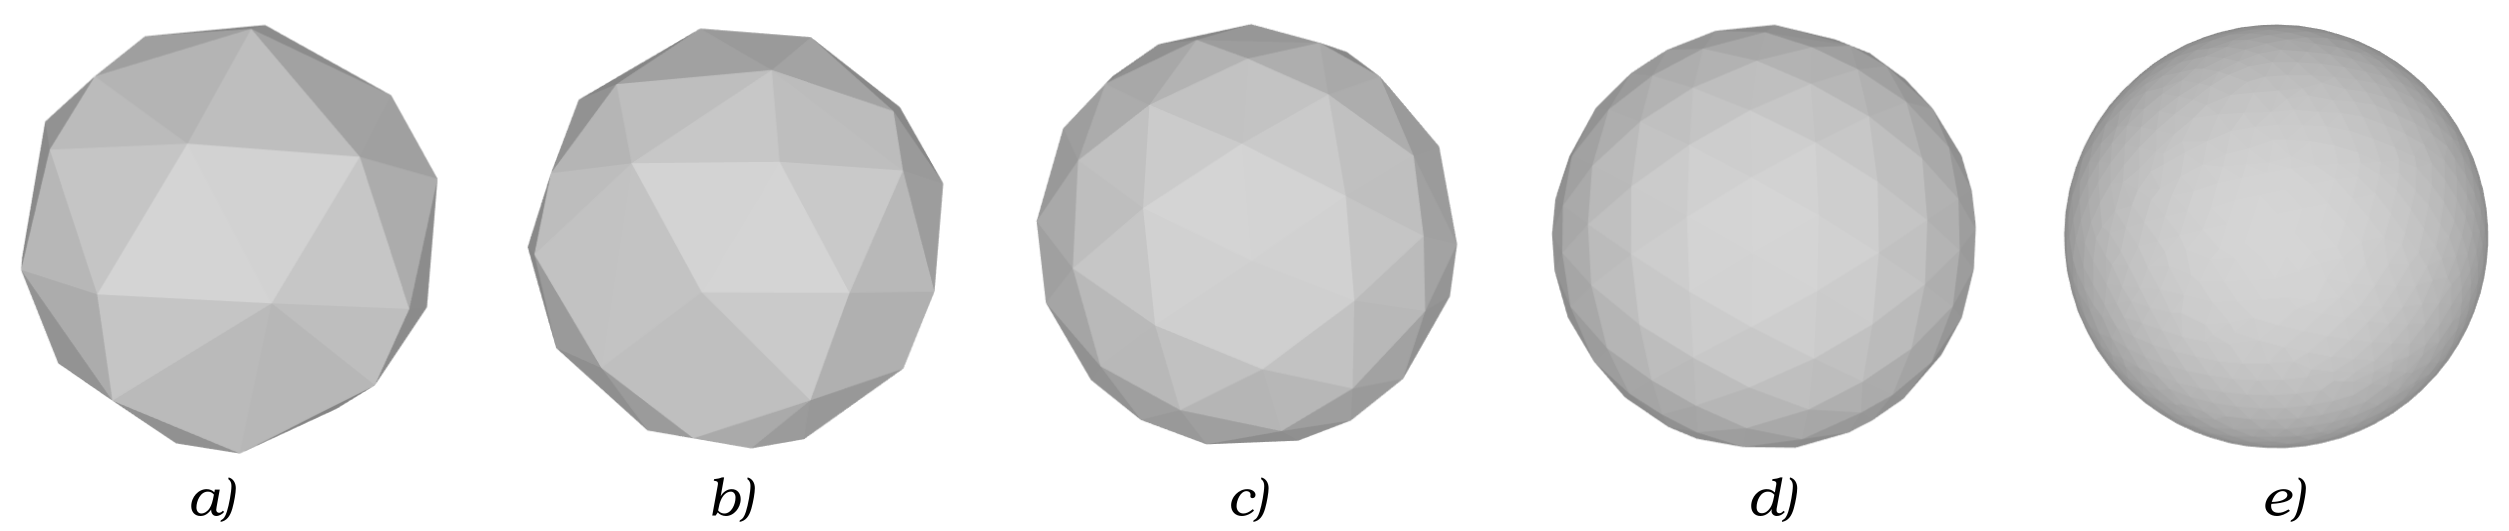
\includegraphics[width=1\textwidth]{images/sphere}}
        \caption[Triangulácia sféry]{Triangulácia sféry.}
        %id obrazku, pomocou ktoreho sa budeme na obrazok odvolavat
        \label{obr:sphere}
    \end{figure}

    Výsledky merania kritérií kvality môžeme vidieť v tabuľke \ref{tab:sphere}.
    
    \renewcommand*{\MinNumberA}{0.725}%
    \renewcommand*{\MaxNumberA}{0.954}%
    \pgfmathsetmacro{\MidNumberA}{(\MinNumberA+\MaxNumberA)/2}%
    \renewcommand*{\MinNumberB}{0.015}%
    \renewcommand*{\MaxNumberB}{0.085}%
    \pgfmathsetmacro{\MidNumberB}{(\MinNumberB+\MaxNumberB)/2}%
    \renewcommand*{\MinNumberC}{1.210}%
    \renewcommand*{\MaxNumberC}{1.305}%
    \pgfmathsetmacro{\MidNumberC}{(\MinNumberC+\MaxNumberC)/2}%
    \renewcommand*{\MinNumberD}{0.028}%
    \renewcommand*{\MaxNumberD}{0.136}%
    \pgfmathsetmacro{\MidNumberD}{(\MinNumberD+\MaxNumberD)/2}%
    \renewcommand*{\MinNumberE}{0.0}%
    \renewcommand*{\MaxNumberE}{5.140}%
    \pgfmathsetmacro{\MidNumberE}{(\MinNumberE+\MaxNumberE)/2}%
    \renewcommand*{\MinNumberF}{0.120}%
    \renewcommand*{\MaxNumberF}{0.646}%
    \pgfmathsetmacro{\MidNumberF}{(\MinNumberF+\MaxNumberF)/2}%
    \renewcommand*{\MinNumberG}{0.720}%
    \renewcommand*{\MaxNumberG}{0.951}%
    \pgfmathsetmacro{\MidNumberG}{(\MinNumberG+\MaxNumberG)/2}%
    \renewcommand*{\MinNumberH}{0.088}%
    \renewcommand*{\MaxNumberH}{0.112}%
    \pgfmathsetmacro{\MidNumberH}{(\MinNumberH+\MaxNumberH)/2}%


    \begin{table}[ht]
    \caption[Výsledky merania triangulácie sféry]{Výsledky merania}
        \begin{center}
        \label{tab:sphere}
            \begin{tabular}{| c |ABCDEFGH|}
                \hline
                \hline
                \multicolumn{9}{|c|}{Sféra} \\
                \hline
                \hline
                $\hspace{8mm} a \hspace{8mm}$ & $k_1$ & $k_2$ & $k_3$ & $k_4$ & $k_5$ & $k_6$ & $k_7$ & $k_8$ \EndTableHeader\\
                \hline
                \hline
                0.900 & 0.725 & 0.085 & 1.305 & 0.136 & 1.380 & 0.646 & 0.720 & 0.100 \\
                \hline
                0.700 & 0.798 & 0.079 & 1.321 & 0.131 & 0.000 & 0.617 & 0.792 & 0.112 \\
                \hline
                0.500 & 0.847 & 0.062 & 1.253 & 0.104 & 5.140 & 0.472 & 0.843 & 0.097 \\
                \hline
                0.300 & 0.895 & 0.041 & 1.274 & 0.074 & 0.005 & 0.291 & 0.892 & 0.103 \\
                \hline
                0.100 & 0.954 & 0.015 & 1.210 & 0.028 & 0.066 & 0.120 & 0.951 & 0.088 \\
                \hline
                \hline
            \end{tabular}
        \end{center}
    \end{table}

}

\newpage

\item{
    \textit{Elipsoid}
    \begin{equation}
    \label{eq:ellipsoid}
        \bigg ( \frac{x-1}{2} \bigg )^2 + \bigg (\frac{y-1}{3} \bigg )^2 + (z - 1)^2 - 1 = 0
    \end{equation}

    Na obrázku \ref{obr:ellipsoid} vidíme výslednú trianguláciu elipsoidu daného implicitnou 
    rovnicou \ref{eq:ellipsoid} s piatimi rôznymi dĺžkami strany $a$.
    \begin{enumerate}[a)]
    \item{
        $a=0.900$, $n=214$, $p=109$
    }
    \item{
        $a=0.700$, $n=332$, $p=168$
    }
    \item{
        $a=0.500$, $n=574$, $p=289$
    }
    \item{
        $a=0.300$, $n=1460$, $p=732$
    }
    \item{
        $a=0.150$, $n=5476$, $p=2740$
    }
    \end{enumerate}

    \begin{figure}
        \centerline{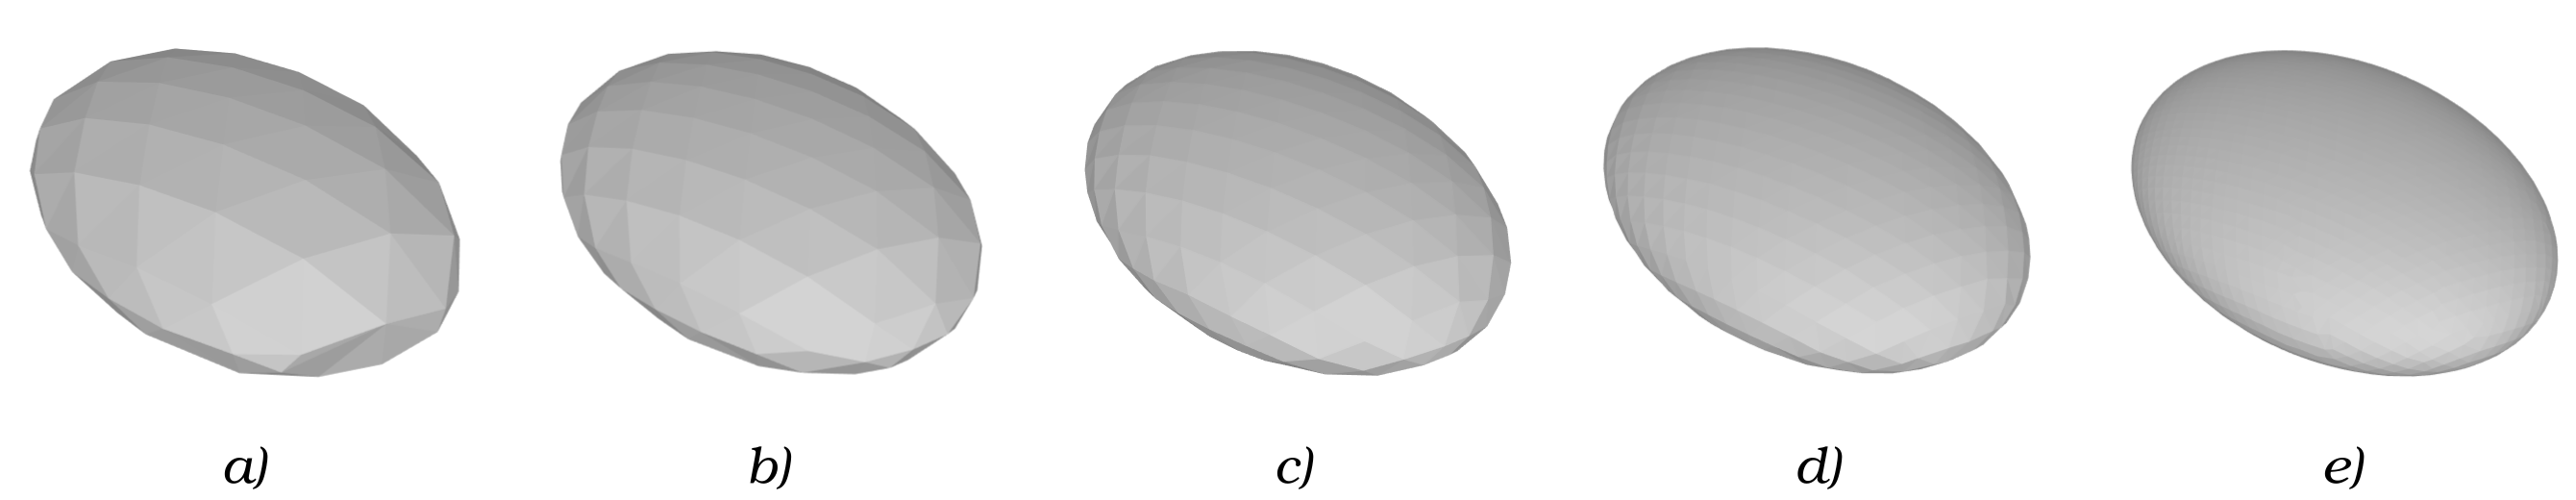
\includegraphics[width=1\textwidth]{images/ellipsoid}}
        \caption[Triangulácia elipsoidu]{Triangulácia elipsoidu.}
        %id obrazku, pomocou ktoreho sa budeme na obrazok odvolavat
        \label{obr:ellipsoid}
    \end{figure}

    Výsledky merania kritérií kvality môžeme vidieť v tabuľke \ref{tab:ellipsoid}.

    \renewcommand*{\MinNumberA}{0.802}%
    \renewcommand*{\MaxNumberA}{0.962}%
    \pgfmathsetmacro{\MidNumberA}{(\MinNumberA+\MaxNumberA)/2}%
    \renewcommand*{\MinNumberB}{0.013}%
    \renewcommand*{\MaxNumberB}{0.049}%
    \pgfmathsetmacro{\MidNumberB}{(\MinNumberB+\MaxNumberB)/2}%
    \renewcommand*{\MinNumberC}{1.142}%
    \renewcommand*{\MaxNumberC}{1.356}%
    \pgfmathsetmacro{\MidNumberC}{(\MinNumberC+\MaxNumberC)/2}%
    \renewcommand*{\MinNumberD}{0.057}%
    \renewcommand*{\MaxNumberD}{0.192}%
    \pgfmathsetmacro{\MidNumberD}{(\MinNumberD+\MaxNumberD)/2}%
    \renewcommand*{\MinNumberE}{0.0}%
    \renewcommand*{\MaxNumberE}{0.073}%
    \pgfmathsetmacro{\MidNumberE}{(\MinNumberE+\MaxNumberE)/2}%
    \renewcommand*{\MinNumberF}{0.338}%
    \renewcommand*{\MaxNumberF}{1.122}%
    \pgfmathsetmacro{\MidNumberF}{(\MinNumberF+\MaxNumberF)/2}%
    \renewcommand*{\MinNumberG}{0.796}%
    \renewcommand*{\MaxNumberG}{0.961}%
    \pgfmathsetmacro{\MidNumberG}{(\MinNumberG+\MaxNumberG)/2}%
    \renewcommand*{\MinNumberH}{0.061}%
    \renewcommand*{\MaxNumberH}{0.116}%
    \pgfmathsetmacro{\MidNumberH}{(\MinNumberH+\MaxNumberH)/2}%

    \begin{table}[ht]
    \caption[Výsledky merania triangulácie elipsoidu]{Výsledky merania}
        \begin{center}
        \label{tab:ellipsoid}
            \begin{tabular}{|c|A B C D E F G H|}
                \hline
                \hline
                \multicolumn{9}{|c|}{Elipsoid} \\
                \hline
                \hline
                $\hspace{8mm} a \hspace{8mm}$ & $k_1$ & $k_2$ & $k_3$ & $k_4$ & $k_5$ & $k_6$ & $k_7$ & $k_8$ \EndTableHeader\\
                \hline
                \hline
                0.900 & 0.802 & 0.049 & 1.356 & 0.192 & 
                0.073 & 1.220 & 0.796 & 0.116 \\
                \hline
                0.700 & 0.828 & 0.041 & 1.271 & 0.084 & 
                0.017 & 0.888 & 0.823 & 0.098\\
                \hline
                0.500 & 0.881 & 0.035 & 1.204 & 0.084 & 
                0.039 & 0.745 & 0.881 & 0.083\\
                \hline
                0.300 & 0.928 & 0.024 & 1.169 & 0.093 & 
                0.003 & 0.597 & 0.928 & 0.067\\
                \hline
                0.150 & 0.962 & 0.013 & 1.142 & 0.057 & 
                0.000 & 0.338 & 0.961 & 0.061\\
                \hline
                \hline
            \end{tabular}
        \end{center}
    \end{table}
}


\newpage

\item{
    \textit{Zaoblená kocka}
    \begin{equation}
    \label{eq:cubed_sphere}
        x^4+y^4+z^4-1 = 0
    \end{equation}

    Na obrázku \ref{obr:cubed_sphere} vidíme výslednú trianguláciu zaoblenej kocky danej implicitnou 
    rovnicou \ref{eq:cubed_sphere} s piatimi rôznymi dĺžkami strany $a$.
    \begin{enumerate}[a)]
    \item{
        $a=2.000$, $n=30$, $p=17$
    }
    \item{
        $a=1.000$, $n=68$, $p=36$
    }
    \item{
        $a=0.500$, $n=216$, $p=110$
    }
    \item{
        $a=0.250$, $n=748$, $p=376$
    }
    \item{
        $a=0.150$, $n=2034$, $p=1018$
    }
    \end{enumerate}

    \begin{figure}
        \centerline{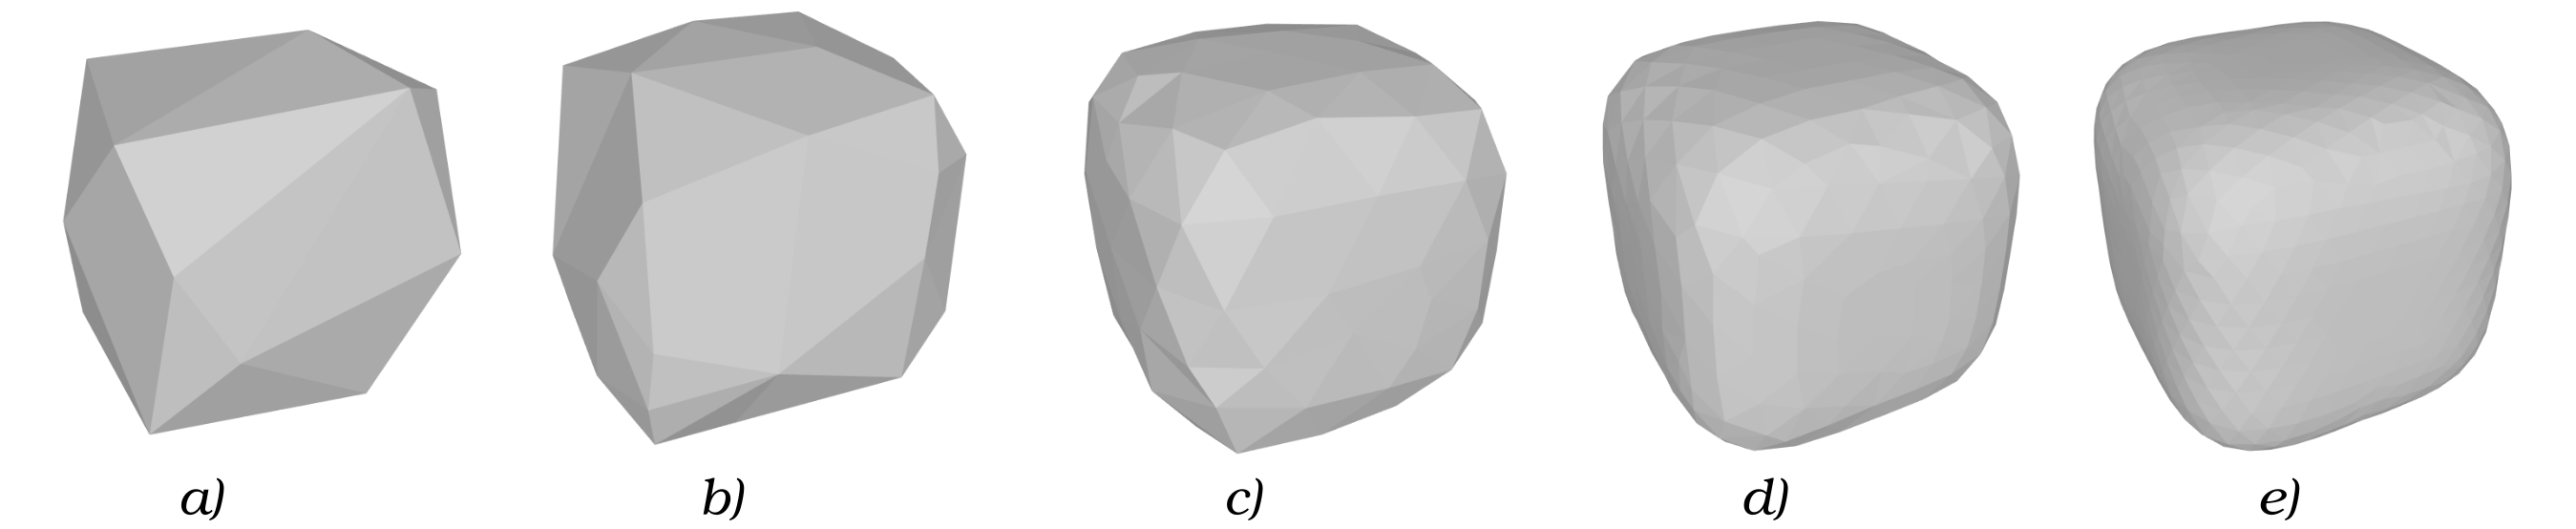
\includegraphics[width=1\textwidth]{images/cubed_sphere}}
        \caption[Triangulácia zaoblenej kocky]{Triangulácia zaoblenej kocky.}
        %id obrazku, pomocou ktoreho sa budeme na obrazok odvolavat
        \label{obr:cubed_sphere}
    \end{figure}

    Výsledky merania kritérií kvality môžeme vidieť v tabuľke \ref{tab:cubed_sphere}.

    \renewcommand*{\MinNumberA}{0.555}%
    \renewcommand*{\MaxNumberA}{0.949}%
    \pgfmathsetmacro{\MidNumberA}{(\MinNumberA+\MaxNumberA)/2}%
    \renewcommand*{\MinNumberB}{0.020}%
    \renewcommand*{\MaxNumberB}{0.077}%
    \pgfmathsetmacro{\MidNumberB}{(\MinNumberB+\MaxNumberB)/2}%
    \renewcommand*{\MinNumberC}{1.189}%
    \renewcommand*{\MaxNumberC}{1.681}%
    \pgfmathsetmacro{\MidNumberC}{(\MinNumberC+\MaxNumberC)/2}%
    \renewcommand*{\MinNumberD}{0.069}%
    \renewcommand*{\MaxNumberD}{0.244}%
    \pgfmathsetmacro{\MidNumberD}{(\MinNumberD+\MaxNumberD)/2}%
    \renewcommand*{\MinNumberE}{0.004}%
    \renewcommand*{\MaxNumberE}{0.524}%
    \pgfmathsetmacro{\MidNumberE}{(\MinNumberE+\MaxNumberE)/2}%
    \renewcommand*{\MinNumberF}{0.348}%
    \renewcommand*{\MaxNumberF}{1.128}%
    \pgfmathsetmacro{\MidNumberF}{(\MinNumberF+\MaxNumberF)/2}%
    \renewcommand*{\MinNumberG}{0.548}%
    \renewcommand*{\MaxNumberG}{0.947}%
    \pgfmathsetmacro{\MidNumberG}{(\MinNumberG+\MaxNumberG)/2}%
    \renewcommand*{\MinNumberH}{0.079}%
    \renewcommand*{\MaxNumberH}{0.152}%
    \pgfmathsetmacro{\MidNumberH}{(\MinNumberH+\MaxNumberH)/2}%
    
     \begin{table}[ht]
     \caption[Výsledky merania triangulácie zaoblenej kocky]{Výsledky merania}
        \begin{center}
        \label{tab:cubed_sphere}
            \begin{tabular}{|c|A B C D E F G H|}
                \hline
                \hline
                \multicolumn{9}{|c|}{Zaoblená kocka} \\
                \hline
                \hline
                $\hspace{8mm} a \hspace{8mm}$ & $k_1$ & $k_2$ & $k_3$ & $k_4$ & $k_5$ & $k_6$ & $k_7$ & $k_8$ \EndTableHeader\\
                \hline
                \hline
                2.000 & 0.555 & 0.066 & 1.681 & 0.143 & 0.482 & 1.228 & 0.548 & 0.136\\
                \hline
                1.000 & 0.750 & 0.077 & 1.454 & 0.244 & 0.524 & 1.062 & 0.738 & 0.152\\
                \hline
                0.500 & 0.865 & 0.051 & 1.286 & 0.173 & 0.040 & 0.837 & 0.861 & 0.111\\
                \hline
                0.250 & 0.935 & 0.031 & 1.189 & 0.099 & 0.026 & 0.591 & 0.932 & 0.080\\
                \hline
                0.150 & 0.949 & 0.020 & 1.189 & 0.069 & 0.004 & 0.348 & 0.947 & 0.079\\
                \hline
                \hline
            \end{tabular}
        \end{center}
    \end{table}
}

\newpage

\item{
    \textit{Torus}
    \begin{equation}
    \label{eq:torus}
        (x^2+y^2+z^2+1375)^2-6400(x^2+y^2) = 0
    \end{equation}

    Na obrázku \ref{obr:torus} vidíme výslednú trianguláciu torusu daného implicitnou 
    rovnicou \ref{eq:torus} s piatimi rôznymi dĺžkami strany $a$.
    \begin{enumerate}[a)]
    \item{
        $a=15$, $n=334$, $p=167$
    }
    \item{
        $a=12$, $n=494$, $p=247$
    }
    \item{
        $a=9$, $n=818$, $p=409$
    }
    \item{
        $a=6$, $n=1720$, $p=860$
    }
    \item{
        $a=3$, $n=6596$, $p=3297$
    }
    \end{enumerate}

    \begin{figure}
        \centerline{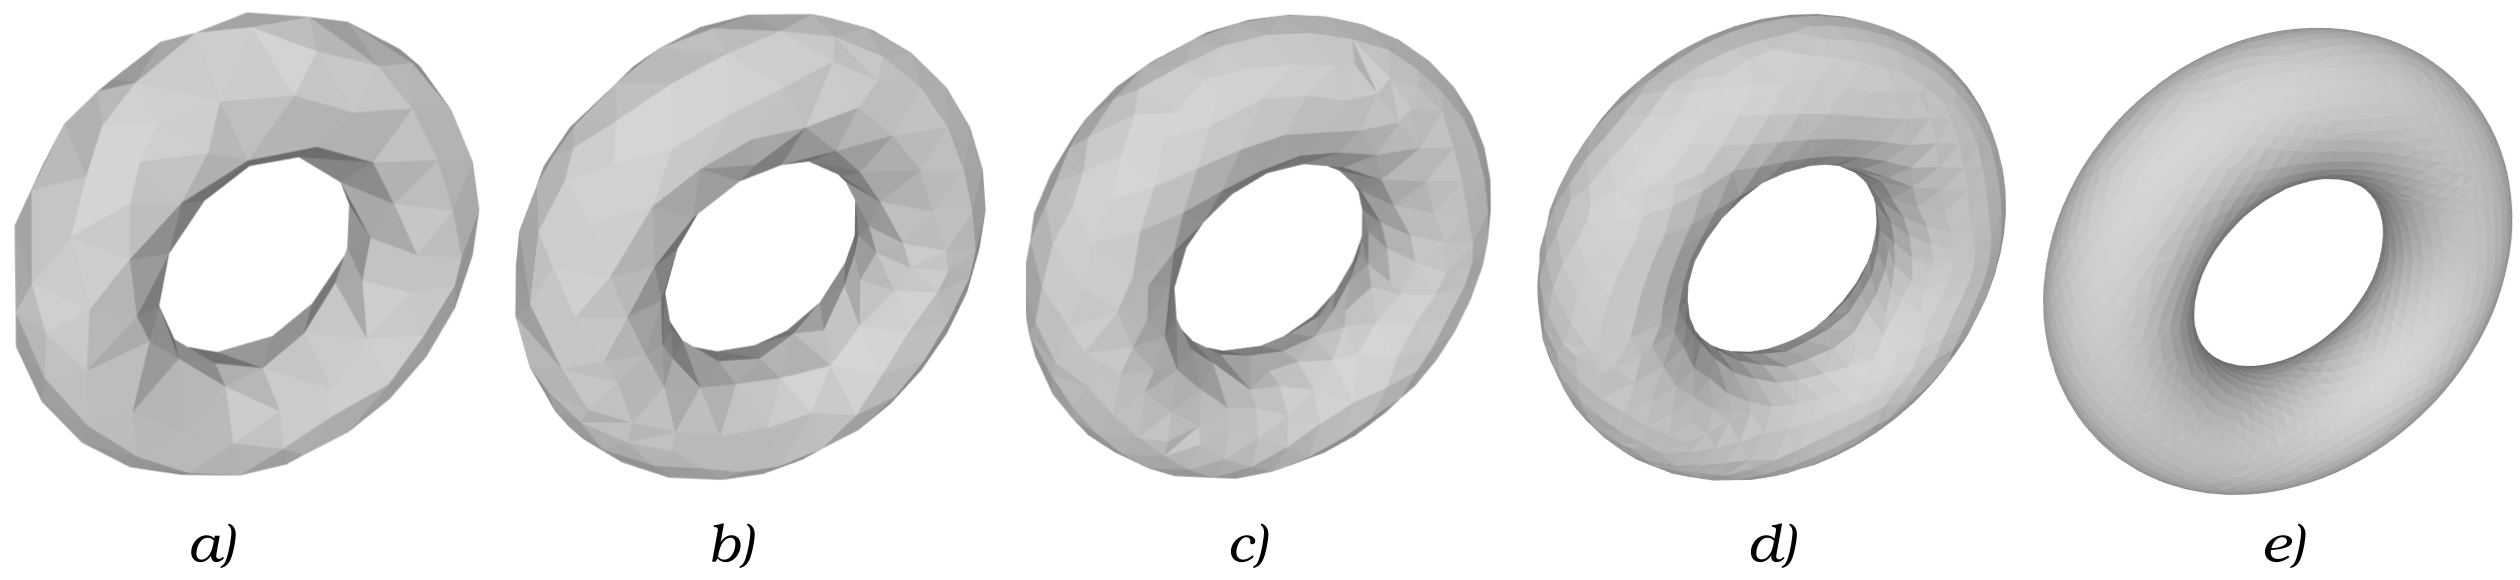
\includegraphics[width=1\textwidth]{images/torus}}
        \caption[Triangulácia torusu]{Triangulácia torusu.}
        %id obrazku, pomocou ktoreho sa budeme na obrazok odvolavat
        \label{obr:torus}
    \end{figure}

    Výsledky merania kritérií kvality môžeme vidieť v tabuľke \ref{tab:torus}.

     
    \renewcommand*{\MinNumberA}{0.856}%
    \renewcommand*{\MaxNumberA}{0.968}%
    \pgfmathsetmacro{\MidNumberA}{(\MinNumberA+\MaxNumberA)/2}%
    \renewcommand*{\MinNumberB}{0.016}%
    \renewcommand*{\MaxNumberB}{0.060}%
    \pgfmathsetmacro{\MidNumberB}{(\MinNumberB+\MaxNumberB)/2}%
    \renewcommand*{\MinNumberC}{1.197}%
    \renewcommand*{\MaxNumberC}{1.331}%
    \pgfmathsetmacro{\MidNumberC}{(\MinNumberC+\MaxNumberC)/2}%
    \renewcommand*{\MinNumberD}{0.052}%
    \renewcommand*{\MaxNumberD}{0.188}%
    \pgfmathsetmacro{\MidNumberD}{(\MinNumberD+\MaxNumberD)/2}%
    \renewcommand*{\MinNumberE}{0.000}%
    \renewcommand*{\MaxNumberE}{0.067}%
    \pgfmathsetmacro{\MidNumberE}{(\MinNumberE+\MaxNumberE)/2}%
    \renewcommand*{\MinNumberF}{0.467}%
    \renewcommand*{\MaxNumberF}{0.974}%
    \pgfmathsetmacro{\MidNumberF}{(\MinNumberF+\MaxNumberF)/2}%
    \renewcommand*{\MinNumberG}{0.851}%
    \renewcommand*{\MaxNumberG}{0.966}%
    \pgfmathsetmacro{\MidNumberG}{(\MinNumberG+\MaxNumberG)/2}%
    \renewcommand*{\MinNumberH}{0.083}%
    \renewcommand*{\MaxNumberH}{0.117}%
    \pgfmathsetmacro{\MidNumberH}{(\MinNumberH+\MaxNumberH)/2}%

  
     \begin{table}[ht]
     \caption[Výsledky merania triangulácie torusu]{Výsledky merania}
        \begin{center}
        \label{tab:torus}
            \begin{tabular}{|c|A B C D E F G H|}
                \hline
                \hline
                \multicolumn{9}{|c|}{Torus} \\
                \hline
                \hline
                $\hspace{5mm} a \hspace{5mm}$ & $k_1$ & $k_2$ & $k_3$ & $k_4$ & $k_5$ & $k_6$ & $k_7$ & $k_8$ \EndTableHeader\\
                \hline
                \hline
                15 & 0.856 & 0.060 & 1.324 & 0.188 & 0.000 & 0.974 & 0.851 & 0.116\\
                \hline
                12 & 0.882 & 0.051 & 1.331 & 0.151 & 0.067 & 0.823 & 0.878 & 0.117\\
                \hline
                9 & 0.916 & 0.042 & 1.284 & 0.097 & 0.013 & 0.671 & 0.912 & 0.109\\
                \hline
                6 & 0.946 & 0.030 & 1.227 & 0.078 & 0.001 & 0.467 & 0.944 & 0.094\\
                \hline
                3 & 0.968 & 0.016 & 1.197 & 0.052 & 0.002 & 0.868 & 0.966 & 0.083\\
                \hline
                \hline
            \end{tabular}
        \end{center}
    \end{table}

}

\newpage

\item{
    \textit{Genus}
    \begin{equation}
    \label{eq:genus}
        2y(y^2-3x^2)(1-z^2)+(x^2+y^2)^2-(9z^2-1)(1-z^2) = 0
    \end{equation}

    Na obrázku \ref{obr:genus} vidíme výslednú trianguláciu genusu daného implicitnou 
    rovnicou \ref{eq:genus} s piatimi rôznymi dĺžkami strany $a$.
    \begin{enumerate}[a)]
    \item{
        $a=0.225$, $n=1566$, $p=781$
    }
    \item{
        $a=0.200$, $n=1958$, $p=977$
    }
    \item{
        $a=0.175$, $n=2480$, $p=1238$
    }
    \item{
        $a=0.150$, $n=3330$, $p=1663$
    }
    \item{
        $a=0.125$, $n=4614$, $p=2305$
    }
    \end{enumerate}

    \begin{figure}
        \centerline{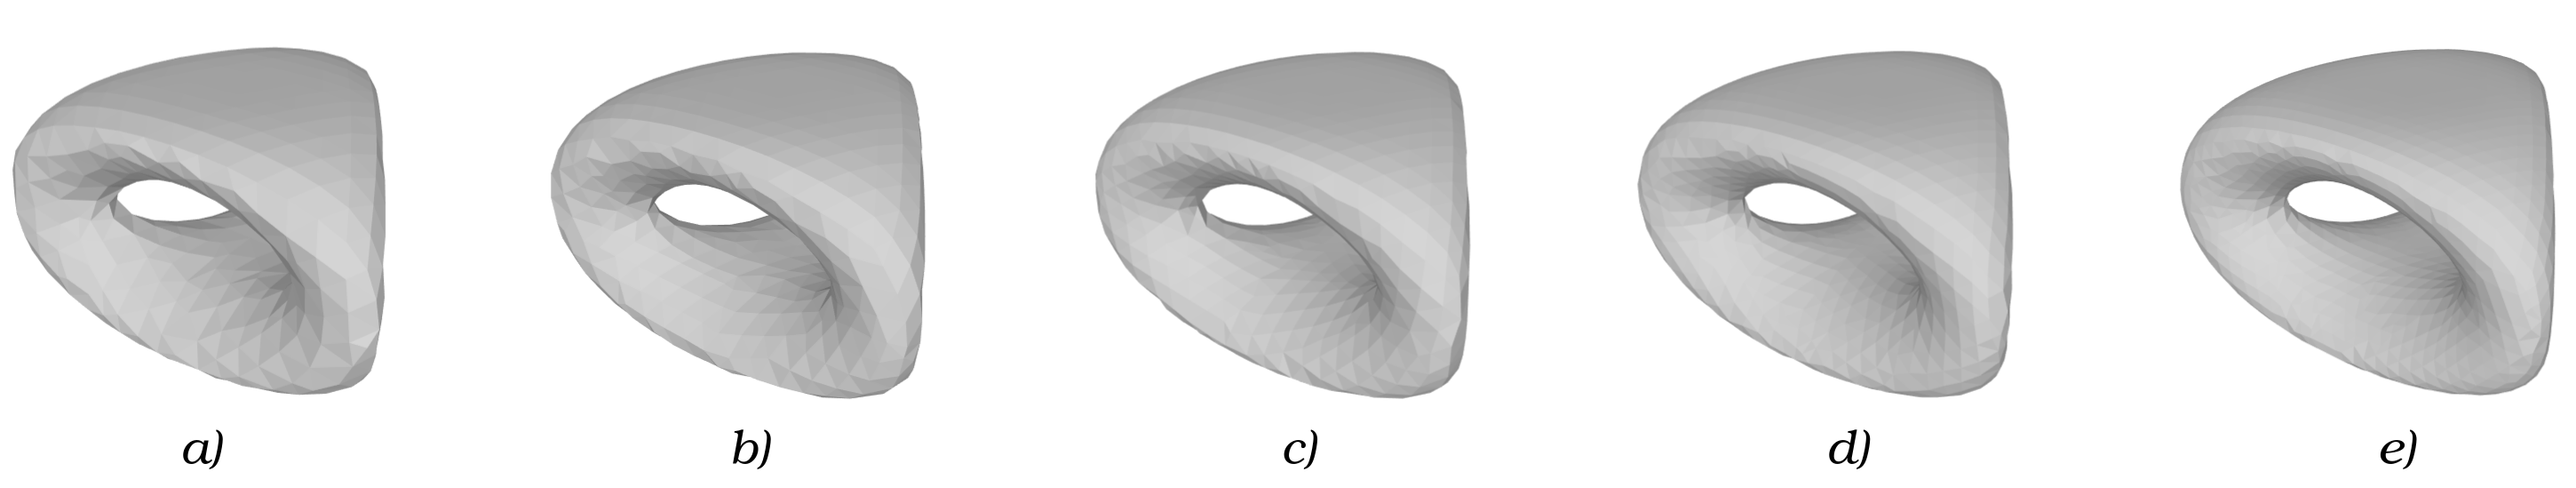
\includegraphics[width=1\textwidth]{images/genus}}
        \caption[Triangulácia genusu]{Triangulácia genusu.}
        %id obrazku, pomocou ktoreho sa budeme na obrazok odvolavat
        \label{obr:genus}
    \end{figure}

    Výsledky merania kritérií kvality môžeme vidieť v tabuľke \ref{tab:genus}.

    \renewcommand*{\MinNumberA}{0.912}%
    \renewcommand*{\MaxNumberA}{0.954}%
    \pgfmathsetmacro{\MidNumberA}{(\MinNumberA+\MaxNumberA)/2}%
    \renewcommand*{\MinNumberB}{0.018}%
    \renewcommand*{\MaxNumberB}{0.029}%
    \pgfmathsetmacro{\MidNumberB}{(\MinNumberB+\MaxNumberB)/2}%
    \renewcommand*{\MinNumberC}{1.223}%
    \renewcommand*{\MaxNumberC}{1.303}%
    \pgfmathsetmacro{\MidNumberC}{(\MinNumberC+\MaxNumberC)/2}%
    \renewcommand*{\MinNumberD}{0.099}%
    \renewcommand*{\MaxNumberD}{0.307}%
    \pgfmathsetmacro{\MidNumberD}{(\MinNumberD+\MaxNumberD)/2}%
    \renewcommand*{\MinNumberE}{0.001}%
    \renewcommand*{\MaxNumberE}{0.005}%
    \pgfmathsetmacro{\MidNumberE}{(\MinNumberE+\MaxNumberE)/2}%
    \renewcommand*{\MinNumberF}{0.896}%
    \renewcommand*{\MaxNumberF}{2.716}%
    \pgfmathsetmacro{\MidNumberF}{(\MinNumberF+\MaxNumberF)/2}%
    \renewcommand*{\MinNumberG}{0.907}%
    \renewcommand*{\MaxNumberG}{0.951}%
    \pgfmathsetmacro{\MidNumberG}{(\MinNumberG+\MaxNumberG)/2}%
    \renewcommand*{\MinNumberH}{0.092}%
    \renewcommand*{\MaxNumberH}{0.114}%
    \pgfmathsetmacro{\MidNumberH}{(\MinNumberH+\MaxNumberH)/2}%

    \begin{table}[ht]
     \caption[Výsledky merania triangulácie genusu]{Výsledky merania}
        \begin{center}
        \label{tab:genus}
            \begin{tabular}{|c|A B C D E F G H|}
                \hline
                \hline
                \multicolumn{9}{|c|}{Genus} \\
                \hline
                \hline
                $\hspace{8mm} a \hspace{8mm}$ & $k_1$ & $k_2$ & $k_3$ & $k_4$ & $k_5$ & $k_6$ & $k_7$ & $k_8$ \EndTableHeader\\
                \hline
                \hline
                0.225 & 0.912 & 0.029 & 1.301 & 0.153 & 0.005 & 1.405 & 0.907 & 0.114\\
                \hline
                0.200 & 0.918 & 0.027 & 1.303 & 0.307 & 0.001 & 2.716 & 0.913 & 0.112\\
                \hline
                0.175 & 0.931 & 0.024 & 1.262 & 0.203 & 0.002 & 1.141 & 0.927 & 0.103\\
                \hline
                0.150 & 0.937 & 0.021 & 1.266 & 0.185 & 0.001 & 0.968 & 0.933 & 0.104\\
                \hline
                0.125 & 0.954 & 0.018 & 1.223 & 0.099 & 0.001 & 0.896 & 0.951 & 0.092\\
                \hline
                \hline
            \end{tabular}
        \end{center}
    \end{table}

}
\end{enumerate}
\section{Nekonečné plochy}
\newpage
\begin{enumerate}
\item{
    \textit{Hyperbolický paraboloid}

    \begin{equation}
    \label{eq:hyperbolic_paraboloid}
        x^2-y^2+2z = 0
    \end{equation}

    Plocha je ohraničená ohraničujúcou obálkou danou $3$-rozmerným intervalom 
    \newline
    \mbox{$\langle -3, 3 \rangle \times \langle -3, 3 \rangle \times \langle -20, 20 \rangle$}.

    Na obrázku \ref{obr:hyperbolic_paraboloid} vidíme výslednú trianguláciu hyperbolického paraboloidu
    daného implicitnou rovnicou \ref{eq:hyperbolic_paraboloid} so štyrmi rôznymi dĺžkami strany $a$.
    \begin{enumerate}[a)]
    \item{
        $a=1.000$, $n=205$, $p=121$
    }
    \item{
        $a=0.750$, $n=380$, $p=218$
    }
    \item{
        $a=0.500$, $n=845$, $p=464$
    }
    \item{
        $a=0.250$, $n=3359$, $p=1767$
    }
    \end{enumerate}

    \begin{figure}
        \centerline{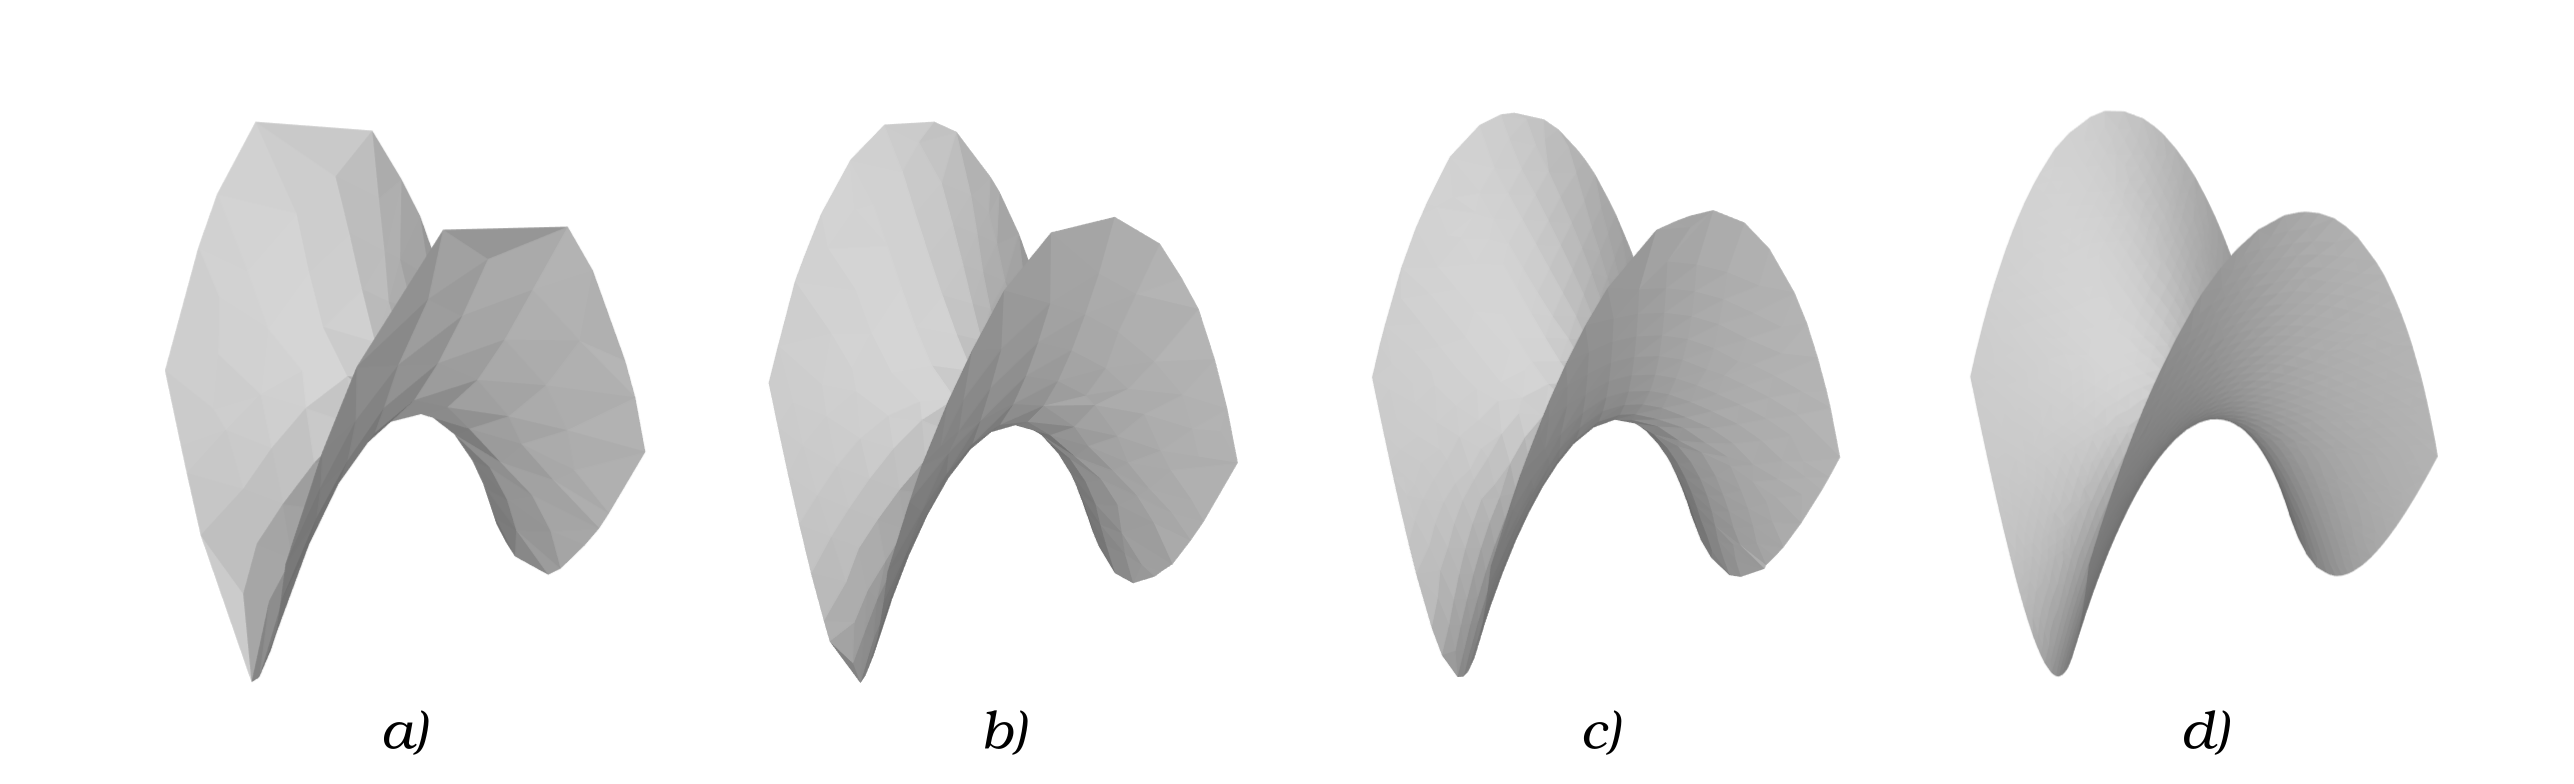
\includegraphics[width=1\textwidth]{images/hyperbolic_paraboloid}}
        \caption[Triangulácia hyperbolického paraboloidu]{Triangulácia hyperbolického paraboloidu.}
        %id obrazku, pomocou ktoreho sa budeme na obrazok odvolavat
        \label{obr:hyperbolic_paraboloid}
    \end{figure}

    Výsledky merania kritérií kvality môžeme vidieť v tabuľke \ref{tab:hyperbolic_paraboloid}.

    \renewcommand*{\MinNumbera}{1.014}%
    \renewcommand*{\MaxNumbera}{1.046}%
    \pgfmathsetmacro{\MidNumbera}{(\MinNumbera+\MaxNumbera)/2}%
    \renewcommand*{\MinNumberB}{0.004}%
    \renewcommand*{\MaxNumberB}{0.017}%
    \pgfmathsetmacro{\MidNumberB}{(\MinNumberB+\MaxNumberB)/2}%
    \renewcommand*{\MinNumberC}{1.209}%
    \renewcommand*{\MaxNumberC}{1.363}%
    \pgfmathsetmacro{\MidNumberC}{(\MinNumberC+\MaxNumberC)/2}%
    \renewcommand*{\MinNumberD}{0.022}%
    \renewcommand*{\MaxNumberD}{0.144}%
    \pgfmathsetmacro{\MidNumberD}{(\MinNumberD+\MaxNumberD)/2}%
    \renewcommand*{\MinNumberE}{0.002}%
    \renewcommand*{\MaxNumberE}{0.032}%
    \pgfmathsetmacro{\MidNumberE}{(\MinNumberE+\MaxNumberE)/2}%
    \renewcommand*{\MinNumberF}{0.520}%
    \renewcommand*{\MaxNumberF}{1.259}%
    \pgfmathsetmacro{\MidNumberF}{(\MinNumberF+\MaxNumberF)/2}%
    \renewcommand*{\MinNumberg}{1.011}%
    \renewcommand*{\MaxNumberg}{1.056}%
    \pgfmathsetmacro{\MidNumberg}{(\MinNumberg+\MaxNumberg)/2}%
    \renewcommand*{\MinNumberH}{0.104}%
    \renewcommand*{\MaxNumberH}{0.200}%
    \pgfmathsetmacro{\MidNumberH}{(\MinNumberH+\MaxNumberH)/2}%


    \begin{table}[ht]
     \caption[Výsledky merania triangulácie hyperbolického paraboloidu]{Výsledky merania}
        \begin{center}
        \label{tab:hyperbolic_paraboloid}
            \begin{tabular}{|c|a B C D E F g H|}
                \hline
                \hline
                \multicolumn{9}{|c|}{Hyperbolický paraboloid} \\
                \hline
                \hline
                $\hspace{8mm} a \hspace{8mm}$ & $k_1$ & $k_2$ & $k_3$ & $k_4$ & $k_5$ & $k_6$ & $k_7$ & $k_8$ \EndTableHeader\\
                \hline
                \hline
                1.000 & 1.046 & 0.017 & 1.363 & 0.144 & 0.010 & 0.860 & 1.056 & 0.200\\
                \hline
                0.750 & 1.015 & 0.011 & 1.313 & 0.095 & 0.032 & 1.259 & 1.012 & 0.160\\
                \hline
                0.500 & 1.016 & 0.008 & 1.259 & 0.040 & 0.006 & 0.520 & 1.013 & 0.132\\
                \hline
                0.250 & 1.014 & 0.004 & 1.209 & 0.022 & 0.002 & 1.072 & 1.011 & 0.104\\
                \hline
                \hline
            \end{tabular}
        \end{center}
    \end{table}
}

\newpage
\item{
    \textit{Regulárna časť kužeľa}

    \begin{equation}
    \label{eq:quadric_cone}
        x^2+y^2-z^2 = 0
    \end{equation}

    Plocha je ohraničená ohraničujúcou obálkou danou $3$-rozmerným intervalom 
    \newline
    \mbox{$\langle -10, 10 \rangle \times \langle -10, 10 \rangle \times \langle 1, 5 \rangle$}.

    Na obrázku \ref{obr:quadric_cone} vidíme výslednú trianguláciu regulárnej časti kužeľa
    daného implicitnou rovnicou \ref{eq:quadric_cone} so štyrmi rôznymi dĺžkami strany $a$.
    \begin{enumerate}[a)]
    \item{
        $a=1.000$, $n=274$, $p=156$
    }
    \item{
        $a=0.750$, $n=462$, $p=254$
    }
    \item{
        $a=0.500$, $n=1012$, $p=541$
    }
    \item{
        $a=0.250$, $n=4041$, $p=2100$
    }
    \end{enumerate}

    \begin{figure}
        \centerline{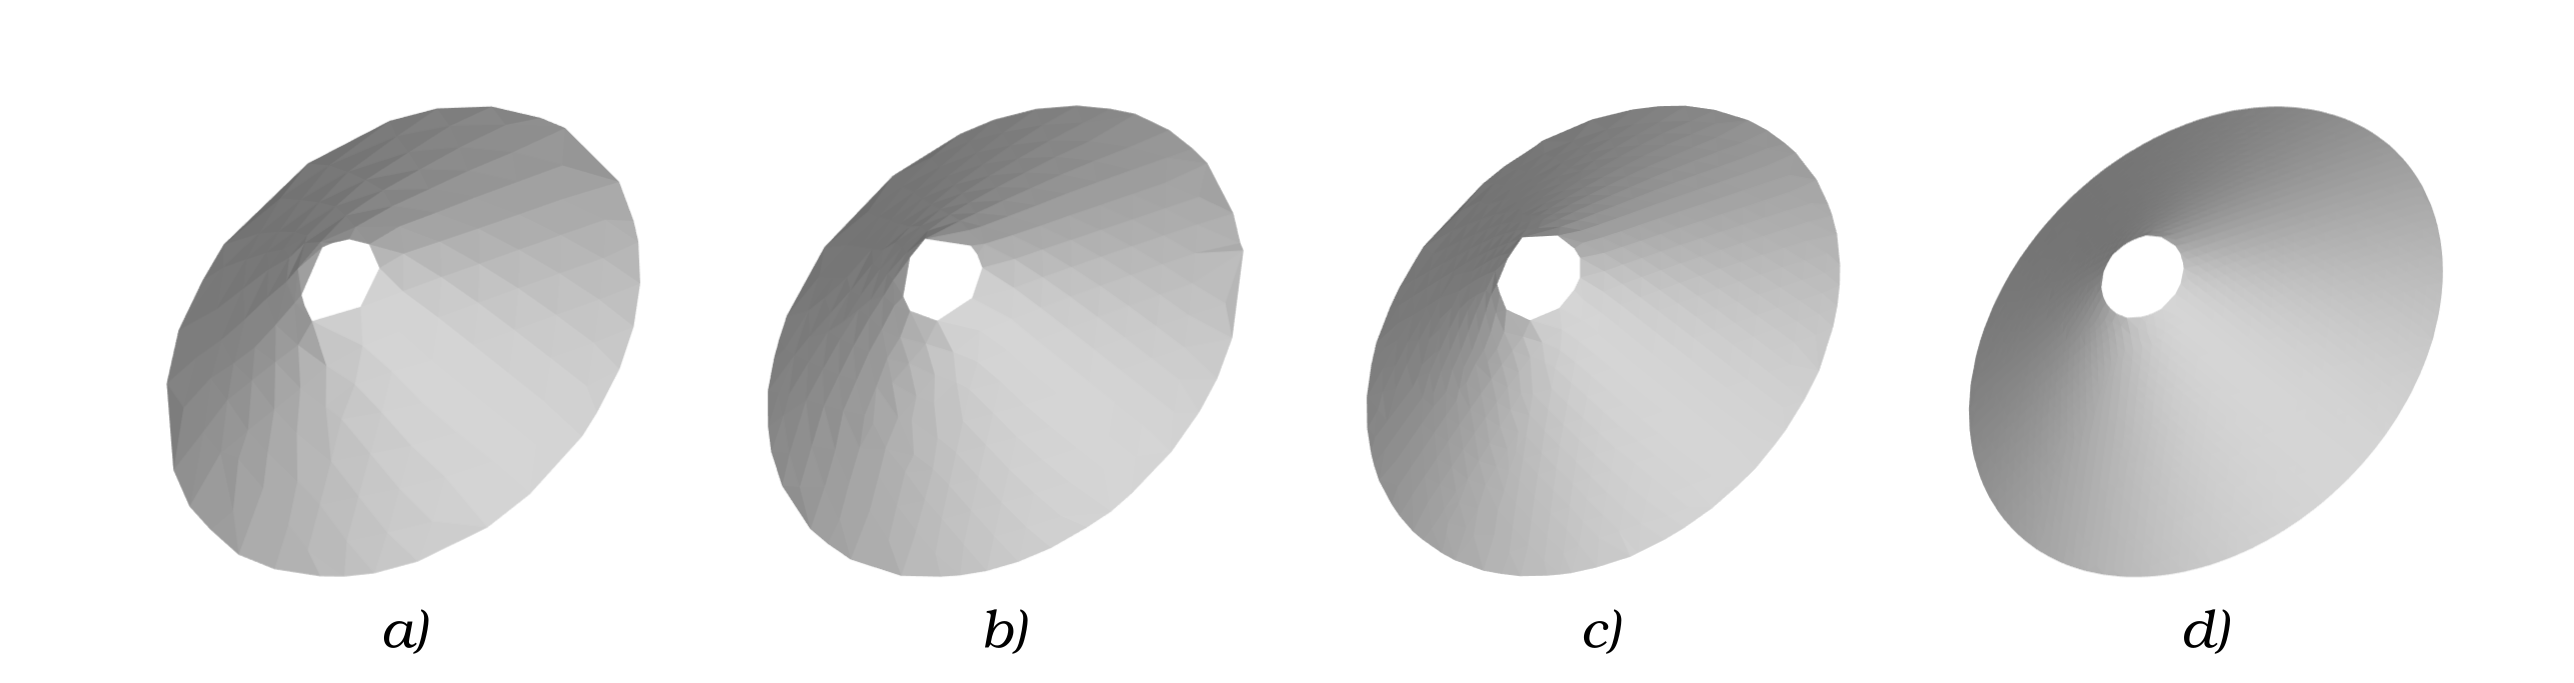
\includegraphics[width=1\textwidth]{images/quadric_cone}}
        \caption[Triangulácia regulárnej časti kužeľa]{Triangulácia regulárnej časti kužeľa.}
        %id obrazku, pomocou ktoreho sa budeme na obrazok odvolavat
        \label{obr:quadric_cone}
    \end{figure}

    Výsledky merania kritériu kvality môžeme vidieť v tabuľke \ref{tab:quadric_cone}.

    \renewcommand*{\MinNumberA}{0.960}%
    \renewcommand*{\MaxNumberA}{0.998}%
    \pgfmathsetmacro{\MidNumberA}{(\MinNumberA+\MaxNumberA)/2}%
    \renewcommand*{\MinNumberB}{0.005}%
    \renewcommand*{\MaxNumberB}{0.020}%
    \pgfmathsetmacro{\MidNumberB}{(\MinNumberB+\MaxNumberB)/2}%
    \renewcommand*{\MinNumberC}{1.114}%
    \renewcommand*{\MaxNumberC}{1.247}%
    \pgfmathsetmacro{\MidNumberC}{(\MinNumberC+\MaxNumberC)/2}%
    \renewcommand*{\MinNumberD}{0.042}%
    \renewcommand*{\MaxNumberD}{0.129}%
    \pgfmathsetmacro{\MidNumberD}{(\MinNumberD+\MaxNumberD)/2}%
    \renewcommand*{\MinNumberE}{0.000}%
    \renewcommand*{\MaxNumberE}{0.041}%
    \pgfmathsetmacro{\MidNumberE}{(\MinNumberE+\MaxNumberE)/2}%
    \renewcommand*{\MinNumberF}{0.196}%
    \renewcommand*{\MaxNumberF}{3.127}%
    \pgfmathsetmacro{\MidNumberF}{(\MinNumberF+\MaxNumberF)/2}%
    \renewcommand*{\MinNumberG}{0.954}%
    \renewcommand*{\MaxNumberG}{0.997}%
    \pgfmathsetmacro{\MidNumberG}{(\MinNumberG+\MaxNumberG)/2}%
    \renewcommand*{\MinNumberH}{0.055}%
    \renewcommand*{\MaxNumberH}{0.121}%
    \pgfmathsetmacro{\MidNumberH}{(\MinNumberH+\MaxNumberH)/2}%

    \begin{table}[ht]
     \caption[Výsledky merania triangulácie regulárnej časti kužeľa]{Výsledky merania}
        \begin{center}
        \label{tab:quadric_cone}
            \begin{tabular}{|c|A B C D E F G H|}
                \hline
                \hline
                \multicolumn{9}{|c|}{Kužeľ} \\
                \hline
                \hline
                $\hspace{8mm} a \hspace{8mm}$ & $k_1$ & $k_2$ & $k_3$ & $k_4$ & $k_5$ & $k_6$ & $k_7$ & $k_8$ \EndTableHeader\\
                \hline
                \hline
                1.000 & 0.960 & 0.020 & 1.247 & 0.129 & 0.026 & 0.491 & 0.954 & 0.121\\
                \hline
                0.750 & 0.988 & 0.014 & 1.209 & 0.110 & 0.041 & 0.414 & 0.986 & 0.108\\
                \hline
                0.500 & 0.998 & 0.009 & 1.181 & 0.055 & 0.003 & 3.127 & 0.997 & 0.093\\
                \hline
                0.250 & 0.992 & 0.005 & 1.114 & 0.042 & 0.000 & 0.196 & 0.988 & 0.055\\
                \hline
                \hline
            \end{tabular}
        \end{center}
    \end{table}
}
\end{enumerate}
